%\documentclass[11pt,a4paper]{jsarticle}                    
\documentclass[11pt,a4paper,uplatex]{ujreport}
% fir platex
%\documentclass[11pt,a4paper,uplatex]{ujreport} 	% for uplatex
%
\usepackage{amsmath,amssymb}
\usepackage{bm}
\usepackage{graphicx}
\usepackage{ascmac}
\usepackage{float}
\usepackage{here}
\usepackage{listings,jvlisting}
%


\newcommand{\argmax}{\mathop{\rm arg~max}\limits}
\newcommand{\argmin}{\mathop{\rm arg~min}\limits}


\lstset{
  basicstyle={\ttfamily},
  identifierstyle={\small},
  commentstyle={\smallitshape},
  keywordstyle={\small\bfseries},
  ndkeywordstyle={\small},
  stringstyle={\small\ttfamily},
  frame={tb},
  breaklines=true,
  columns=[l]{fullflexible},
  numbers=left,
  xrightmargin=0zw,
  xleftmargin=3zw,
  numberstyle={\scriptsize},
  stepnumber=1,
  numbersep=1zw,
  lineskip=-0.5ex
}

\setlength{\textheight}{40\baselineskip}
\addtolength{\textheight}{\topskip}
\setlength{\voffset}{-0.2in}
\setlength{\topmargin}{0pt}
\setlength{\headheight}{0pt}
\setlength{\headsep}{0pt}

\setlength{\textwidth}{\paperwidth}     % ひとまず紙面を本文領域に
\setlength{\oddsidemargin}{-5.4truemm}  % 左の余白を20mm(=1inch-5.4mm)に
\setlength{\evensidemargin}{-5.4truemm} % 
\addtolength{\textwidth}{-40truemm}     % 右の余白も20mmに
%
\newcommand{\divergence}{\mathrm{div}\,}  %ダイバージェンス
\newcommand{\grad}{\mathrm{grad}\,}  %グラディエント
\newcommand{\rot}{\mathrm{rot}\,}  %ローテーション
%
\title{脳を学ぶ上で重要な数学シリーズ\\ 発展数学編}
\author{後藤 優仁}
\date{\today}
\begin{document}
\maketitle
%
%
\tableofcontents

\newpage
\chapter{はじめに}
さて,この数学シリーズの中でもこのadvancedはかなり異質で,筆者が脳神経科学を研究する上で関わっていった様々な (あまり一般的ではない) 議論を展開するために必要になった数学的知識をまとめる場です.筆者は脳活動の非線形ダイナミクスの機能的な役割を研究しています.脳は多数の非線形素子が結合した大自由度の力学系とみなすことができ,多様なダイナミクスを示します.計算論的神経科学の観点で,神経系が示す同期,自発活動,誘発活動ダイナミクス,ノイズ誘発同期,...といった様々な現象を捉え,その情報処理メカニズムの解明を試みています.\\

 こうした作業には,信号処理は勿論,非線形ダイナミクス(つまり力学系),情報理論,複雑系,機械学習...多種多様な数学的,理論的知識が求められます.この勉強については終わりがなく,本当に役に立つのかも分かりません.ただ確実に言えるのは,\\
\\
「○○をやっている時の脳は△△領域で~~ ms後に × Hzの波が同期している!!」
\\
\\
なんてことだけ見ていても,脳を理解する事は出来ないということです.その活動が何故大事なのか,その活動を通してどんな処理をしているのか...こうしたところまで理解してこその科学だと,筆者含め計算論的神経科学者たちは考えています.\\
\\
実験的にデータを集めるだけでは理解に至らず,その背景で何が行われているのか,どんな表現がなされているのか.そんなところまで考えないとだよね,というスタンスです.その必要性が分からん,そんなに大事だろうか.そう思う人はユニークな思考実験的論文があるので是非読んでみてください\cite{radio}\cite{Jonas}.
\\
何をもって脳の理解とするか?
\\
この問に答えるのが,有名なマーの3レベルという概念?お話?\cite{mar}です.\\
\begin{itemize}
 \item{計算理論}
 \item{表現とアルゴリズム}
 \item{ハードウェアによる実装}
\end{itemize}

この3段階を踏み,相互に対応付ける事が脳の理解に大切だ,とする話です.計算理論は,我々が脳を使ってどんな「計算」を行っているのか,行っているべきなのか,といった議論.自由エネルギー原理だとかの話,すなわち脳が採用している戦略を考える所です.ハードウェアによる実装は,多くの神経科学者がやっているように脳のどの部分でどんな活動が起きていてといった解剖学・生理学的知見.最後に表現とアルゴリズムは,ハードウェアの実装を使っていかに計算理論で提案された処理を実行するのか,になります.\\
\\
彼に言わせれば,これまで主流の神経科学はハードウェアの実装ばかりだったわけですね.計算理論と表現に関する議論は,無論ありましたがあまり活発ではなかった.
\\
\\
ここから先,どう考えるかは個人の自由だと思います.計算理論や表現についても考えていこうとするか,そんなに色々手を出しても回収しきれないと見切りをつけるか,あるいは他の人が結び付けてくれる事を期待して実験データを提供するに集中するのか...\\
\\
筆者は,計算理論と実装を結ぶ,表現の研究者になりたいと考えた次第です.一番勉強する事が多いような気もしますが,楽しんでやっていきます.\\
\\
長くなりましたが,本書はそんなモチベーションのもと,計算理論やアルゴリズムについて学習したことをまとめていくものにします.なので神経に本当に役立つのか,理解が正しいのか,様々な問題があると思いますが,まあ教科書ではなく筆者のノートだと思って見てください.結構やってみると楽しいです.また本稿はその性質上,随所で本や論文を引用しながら議論を展開していきます.筆者の拙い理解での説明では不十分だったり不適切だったりすることも少なくないはずなので,気になるところは適宜参照してください.\\
\\
ps. なんて最初は考えていましたが,結局その他にも勉強する事が増えてきたのでもはや「その他集」といったキメラになりました.


\chapter{数学的テクニック}
本稿をまとめていくにあたって,basicで解説したような基礎の微分積分や線形代数,統計ではたちうち出来なくなってしまったので,どうしても学習が必要になってしまったもの達をここにまとめておきます.いずれはbasicとかに飛ばされるのかも知れません.

\section{ラグランジュの未定乗数法}
こいつ,本当に色々なところで出てきます.機械学習でも,ICAやCCAなどの手法もそうだし,とにかく「またお前か!」という感じでした.初めて見た時は意味わからんすぎたので飛ばしていましたが,ちゃんと勉強したら案外そんな事もなかったのでまとめます.いやほんと,こいつが出来るようになるだけで大分学習が楽になる気がします.

\subsection{定義と用法}
まず,式を載せてみます.本来は多次元に拡張可能なもののようですが,とりあえずここでは簡単のため2次元で載せます.

\begin{screen}
  \textbf{ラグランジュの未定乗数法}\\
  制約条件$g(x,y) = 0$の元で,$f(x,y)$を最大化する$(x,y)$を求める問題を考えるとき,ラグランジュ乗数$\lambda$を用いてラグランジュ関数$L$を
  \begin{eqnarray}
    \label{eq:lag1}
    L(x,y,\lambda) = f(x,y) - \lambda g(x,y)
  \end{eqnarray}
  と置くと,ある$(x_0,y_0)$が題意の条件を満たすなら,ある$\lambda_0$が存在し,$(x_0, y_0, \lambda_0)$において
  \begin{eqnarray}
    \label{eq:lag2}
    \frac{\partial L}{\partial x} = \frac{\partial L}{\partial y} = \frac{\partial L}{\partial \lambda} = 0
  \end{eqnarray}
  が成り立つ.
\end{screen}

といったようなものです.\\
\\


何言ってるか訳分からんですよね.2変数関数の極大値問題を考えていて,それが分からないから悩んでいる人に対して「じゃあ3変数にしようか!!」とか意味が分からんし,ここで深くは触れないですけど,実際ラグランジュ使って解いたところで,これで出てきた解=最大値(最小値)となるとは限らなくて,あくまで停留点,つまり極値の候補しか分からんという.うーん.意味あるのかそれ...意味わからんし...なんて考えてしまい,勉強をやめていました.しかしこれから確認するように,考え方はシンプルだし,とてもありがたいものです.\\
\\

まず,用語ですがラグランジュの"未定"乗数法というからには,未定ななんらかの値を掛け算して解く方法?みたいに捉えられますね.この未定乗数が$\lambda$の事です.それから,何故未定かって正味$\lambda$の値そのものには興味がないというか,どうでもいいのです.$\lambda$を使って表せるという事実が大事.

\subsection{証明}
さて,まずは式(\ref{eq:lag2})の各項について考えていきます.あえて3つ目,$\partial L/ \partial \lambda =0$から考えていきます.と言っても,計算すればすぐ分かりますので式をどうぞ.

\begin{align}
  \frac{\partial L}{\partial \lambda} &= \frac{\partial(f(x,y) - \lambda g(x,y))}{\partial \lambda} \nonumber\\
  &= \frac{\partial f(x,y)}{\partial \lambda} - \lambda\frac{\partial g(x,y)}{\partial \lambda} \nonumber \\
  &= -g(x,y) = 0
\end{align}

普通に,関数Lを$\lambda$で偏微分するとこうなりますね.これは結局,制約条件である$g(x,y) =0$の言い換えです.特に意味なし.以上!\\
\\

では残りの二つについて,すなわち$\partial L/ \partial x = \partial L/ \partial y = 0$について考えます.同じくLを展開していくと

\begin{align}
  \frac{\partial L}{\partial x} &= \frac{\partial f(x,y)}{\partial x} - \lambda\frac{\partial g(x,y)}{\partial x}=0 \nonumber \\
  &\therefore \frac{\partial f(x,y)}{\partial x} = \lambda \frac{\partial g(x,y)}{\partial x} \\
  \frac{\partial L}{\partial y} &= \frac{\partial f(x,y)}{\partial y} - \lambda\frac{\partial g(x,y)}{\partial y}=0 \nonumber \\
  &\therefore \frac{\partial f(x,y)}{\partial y} = \lambda \frac{\partial g(x,y)}{\partial y} 
\end{align}

と,それぞれ表せます.ただの移項なのでここまでは大丈夫でしょう.そして,でてきたこの二つの式をベクトルの形に整理すると次のようになります.

\begin{align}
  \label{eq:lag3}
  \begin{pmatrix}
    \displaystyle \frac{\partial f(x,y)}{\partial x}\\
    \\
    \displaystyle \frac{\partial f(x,y)}{\partial y}
  \end{pmatrix}
  =\lambda
  \begin{pmatrix}
    \displaystyle \frac{\partial g(x,y)}{\partial y}\\
    \\
    \displaystyle \frac{\partial g(x,y)}{\partial y}
  \end{pmatrix}
\end{align}

綺麗になりました.さて,さらにここで,一般にこれらのように関数をそれぞれの変数で偏微分して並べたやつって勾配($\nabla$)と言うんでした.なので更にこの式(\ref{eq:lag3})を以下のように表します.

\begin{align}
  \nabla f = \lambda \nabla g
\end{align}

さて,この意味するところはfの勾配はgの勾配が$\lambda$倍されたものであるという事になります.勾配とは,その点で取った接線に垂直な線,法線ベクトルを指すんでした.よって,この式の意味するところはfとgの法線ベクトルが定数倍,並行であるという事になります.\\
\\
逆説的になりますが,法線ベクトルが並行という事は,この二つの関数が接している,接線を共有しているという事になります.\\
\\

具体例に戻ります.ある制約条件$g(x,y) = 0$の元,ある一定数kに対して$f(x,y) = k$を満たす$f(x,y)$を考えると,こいつは(x,y)平面上の曲線となり,関数fの等高線ぽいものになります.考えたい問題はfの$g(x,y)$の元での最大化なので,この等高線と制約条件の曲線とがちょうど接する時が極値になります.

何故なら,接しておらず交差している場合,制約条件を満たす範囲に$f(x,y) > k, f(x,y) <k$の領域が存在してしまうためです.それならそっちにずれた方が値が大きく(小さく)なりますよね.制約条件にぎりっぎり引っかかる,かすめる時が極値になっているわけです.ここら辺は普通に微分の考え方ですね.\\
\\

もちろん,単純に$f(x,y)$の接線の傾きが0になる点と,今回求めている点は違います.あくまで$g(x,y)$の範囲の中(というより淵だけど)での話です.そのために二つの曲線の接線が等しくなる点を探すのがラグランジュの未定乗数法でした.

\subsection{例題}
$g(x,y) = x+y-1=0$の制約条件のもと,関数$f(x,y) = 1-x^2-y^2$の最大値を考えてみます.\\
制約条件の元の極値問題なので,ラグランジュの未定乗数法を使います.まずラグランジュ関数Lは以下のようになります.

\begin{align}
  L(x,y,\lambda) = 1-x^2-y^2 -\lambda(x+y-1)
\end{align}

続いて,$x,y,\lambda$のそれぞれについて偏微分すると,

\begin{align}
  \frac{\partial L}{\partial x} = -2x-\lambda =0\\
  \frac{\partial L}{\partial y} = -2y - \lambda=0\\
  \frac{\partial L}{\partial \lambda} = -x - y +1=0
\end{align}

が導けます.この連立方程式を解くと,関数fの制約条件gの元での最大値は$(\frac{1}{2}, \frac{1}{2})$であり,対応するラグランジュ乗数は1である事が分かりました.\\
\\

簡単ですね!!

\chapter{情報理論}
近年は神経科学に情報理論の議論を輸入するのが流行りになっている気がします.脳波の解析もだし,情報処理の理論もそうだし,いろんなとこで見るのでとりあえず勉強.関係する研究は以下とか\\
\begin{itemize}
 \item{自由エネルギー原理\cite{fep}}
 \item{Phase Amplitude Couplingの評価. \cite{tort}}
 \item{相互情報量}
 \item{トランスファーエントロピー}
\end{itemize}
*まだちゃんと引っ張ってきてない
\section{エントロピー}
はじめにエントロピーの考え方を導入しましょう.まずは離散確率変数$x$を考えます.観測者がこの変数に対するある値を観測したとき,どれだけの情報量,surpriseを得られるのか.これを考える概念がエントロピーです.\\
直観的に,起きそうもない事象が得られたら情報量は大きいし,その逆も然りですよね.宝くじで1等があたるのはめちゃくちゃびっくりする,つまり情報量大きいけど,参加賞的なのもらっても何も思いません.つまり情報量は確率分布$p(x)$に依存していて,その値によって定まる単調な関数$h(x)$といえます.\\
\\
また,2つの事象$x, y$を考えたとき,これらが独立なら両方を観測したときの情報量は別個に観測したときの情報量の和と等しい(式\ref{eq:sum})はずです.宝くじが当たる事によるsurpriseによって,帰りに頭に雷が落ちてくる事によって生じるsurpriseが小さくみたいになることはないですよね?あるかもな.ないって事にしてください.\\
よって以下の式(\ref{eq:sum})が成り立ちます.
\begin{eqnarray}
\label{eq:sum}
h(x,y) = h(x) + h(y)
\end{eqnarray}

次に,これらの事象の同時確率についても単純に積で求められます(式\ref{eq:product}).宝くじが当たり,かつ頭に雷が降ってくる確率です.

\begin{eqnarray}
\label{eq:product}
p(x,y) = p(x)p(y)
\end{eqnarray}

もし式(\ref{eq:sum}, \ref{eq:product})が分からないようなら基本的な確率が出来てないので,statistics.pdfで勉強してみてください.\\
\\
さて,ここはちょっとテクいです.\\
\\
この二つの関係から,xとyの確率をかける操作をしたものに対して何らかの処理をしたものが,何らかの処理をしたxとyの和になっているので,関数$h(・)$は対数をとっている事が分かり(ほら,掛け算って対数だと足し算じゃん?),

\begin{eqnarray}
h(x) = -log p(x)
\end{eqnarray}
がいえます.log (x)は単調増加で,確率p(x)は常に0から1の範囲をとるため,$h(x)$の値を常に正にするため符号を反転させている事に注意です.ここで対数の底に2を採用するのが情報理論での一般の使い方で,その場合は$h(x)$の単位はbitになるようです.\\
これを使って,信号のサイズ,情報量(bit)を算出してるわけですね.あとデータの圧縮なんかにも関係するぽいですがそこまでは知らないし触れませんし触れられません.\\
\\
次に,この値を分布全体に適用する事を考えます.つまり,確率分布そのものが与える情報量です.その指標として,確率変数$x$の分布$p(x)$に関して$h(x)=-log p(x)$の期待値をとることで,情報量の平均を定義します.確率変数の期待値の一般的な計算です.これも分からなければやはりstatisticsに行ってください.\\

\begin{eqnarray}
\label{eq:entropy}
H[x] = - \Sigma_{x} p(x) log p(x)
\end{eqnarray}

式(\ref{eq:entropy})に定義する量をシャノンエントロピーといいます\cite{prml}.意外と簡単ですね.もっと難しいと思ってました.\\
\\
ついでにこれを連続変数にすると微分エントロピー(式\ref{eq:entropy2})が求まります.

\begin{eqnarray}
\label{eq:entropy2}
H[x] = - \int p(x) log p(x) dx
\end{eqnarray}

言うまでもないと思いますが,$ \Sigma_{x} p(x)$ も$ \int p(x)$も1です.\\
さて,次に当然浮かぶ疑問は,どんな確率分布だとどんなエントロピーが算出されるのか,です.\\
ちゃんと数学的に証明することも出来るっぽいけど面倒だしそこにあんま興味ないので,simulationしてみます.\\

とりあえず一様分布で確認してみます.0.1から1の値をとる,サンプル数10の一様分布(図\ref{im:ent1})のエントロピーを算出します(コード\ref{sc:ent1}).
\begin{lstlisting}[caption=エントロピーの計算,label=sc:ent1]
x = [0.1:0.1:1];
px = zeros(1,10)+0.1;
H = - sum(x .* log(px));

\end{lstlisting}

\begin{figure}[H]
\label{im:ent1}
  \centering
  \includegraphics[width=15cm]{../figures/dis_entropy1.eps}
  \caption{0.1が10この一様分布}
\end{figure}

エントロピーは12.7でした.次に,同じ一様分布でもサンプル数が多いとどうなるのか試します.先ほどと同じ条件の,100個のデータ(図\ref{im:ent2})です.

\begin{figure}[H]
\label{im:ent2}
  \centering
  \includegraphics[width=15cm]{../figures/dis_entropy2.eps}
  \caption{0.01が100この一様分布}
\end{figure}

エントロピーは232.5. 大きくなりましたね.データ数に応じてエントロピー自体は大きくなるぽいです.\\
次に山を持たせた分布で見てみます.

\begin{figure}[H]
\label{im:ent3}
  \centering
  \includegraphics[width=15cm]{../figures/dis_entropy3.eps}
  \caption{適当につくった山あり分布}
\end{figure}

エントロピーは22.3.一様分布に比べるとかなり小さいです.本当はもっと山の位置動かしたり急峻にさせてみたりと比較したいですが,飽きたので結論.(離散)エントロピーは確率分布$p(x)$が一様分布に近付く程大きくなり,一様分布の時に最大になります.$x * log(x)$なのでまあ,考えればそうかなって感じ.証明は結構めんどくさいぽいです.\\
この性質から,状態の予測が困難であるほどエントロピーが高い事になるので,不確かさ(Uncertainty)の指標として用いられる事が多いですよね.\\
\\
ちなみに微分エントロピーの場合はガウス分布が最もエントロピー高いようです.\\
\\
他にも見れる性質があって,まず$p(x)$が0は困ります.logにかけた時に計算がこわれるので.無限に吹っ飛びます.\\
\\
あと,一様分布の比較から分かるようにデータ数が多いほどエントロピーも増大するぽいですね.これもまあ普通に総和とってるんだから当たり前か?

\section{KL距離}
さて,このエントロピーがどんな事に使えるのか考えていきます.エントロピーは分布の特徴を表す量になっていたわけなので,これを使うと二つの分布の比較,なんてことも出来ることになります.直観的には,全く同じ特徴の分布同士ならそのエントロピーに差はないし,違う分布なら差がある,という感じです.\\
\\
式にしてみましょう.まず,微分エントロピー($- \int p(x) log p(x)$)は確率変数xの分布$p(x)$の元での期待値でした.なら,ここで新しい分布$q(x)$を考えたとき,仮にこの分布が同一($p(x) = q(x)$)であれば,

\begin{eqnarray}
\label{eq:KL1}
  \int p(x) log q(x)dx - \int p(x) log p(x)dx= 0
\end{eqnarray}
が成り立つ事になります.同じ分布の元で考えた同じ確率変数の期待値だから,当たり前です.分布$p(x)$の元で見た$q(x)$の期待値が,分布$p(x)$の元で見た$p(x)$の期待値と等しい,ということです.逆にこの分布が異なるものであるほど,この計算の結果は大きな値を取る事になります.\\
\\
てなわけで,この量をちゃんと正負の調整した上で,「分布$p(x), q(x)$の相対エントロピー,あるいはカルバック-ライブラー距離,またはカルバックライブラーダイバージェンス」として以下の式で定義します\cite{prml}.

\begin{eqnarray}
\label{eq:KLD}
  \mathbb{D}_{KL}(p||q) = - \int p(x) log q(x)dx - (-\int p(x) log p(x)dx)\\
  = -\int p(x) log \frac{q(x)}{p(x)} dx
\end{eqnarray}

一寸ややこしく見えますが,基本的には式(\ref{eq:KL1})をlogについて整理しただけです.\\簡単ですね.\\
\\

KL距離の性質ですが,まず$\mathbb{D}_{KL}(p||q) \geq 0$です.距離だし.\\
等号が成り立つのは分布$p(x), q(x)$が等しいときのみです.\\
\\
それから$\mathbb{D}_{KL}(p||q) \neq \mathbb{D}_{KL}(q||p)$なことにも気を付けてください.分布$p(x)$の元で見た$q(x)$の期待値と, 分布$q(x)$の元でみた$p(x)$の期待値とは別物ですからね.\\
\\
それから,対数なのでKLDは以下のような表記のこともあります.一緒です.logの計算の性質を思い出してください.割り算は引き算です(?)

\begin{eqnarray}
\label{eq:KLD-inv}
  \mathbb{D}_{KL}(p||q) =  \int p(x) log \frac{p(x)}{q(x)} dx
\end{eqnarray}
\\
留意してください.\\
\\
あと,KL ``距離''と日本語で呼んでいますが厳密には距離じゃないので注意が必要です.というのも,KLDは以下に示す距離の公理\cite{distance}を満たしていないからです.\\
\\

\begin{screen}
距離の公理\\
2点A,Bが与えられたとき, 実数$d(A,B)$を与える規則で, 次の性質を満たすものを距離という.
\begin{itemize}
\item{$d(A, B) \geq 0$}
\item{$d(A, B) = 0 \leftrightarrow A=B$}
\item{$d(A, B) = d(B, A)$}
\item{$d(A, B) + d(B, C) \geq d(A, C)$}
\end{itemize}
\end{screen}

このうち,KLDが満たしていないのはなんでしょう?\\
そう,3つめの対称性ですね!$\mathbb{D}_{KL}(p||q) \neq \mathbb{D}_{KL}(q||p)$でした.\\
\\
あと4つ目,三角不等式も怪しいと思うんですよね.呼んでた資料とかでは特に対称性のとこだけネチネチと言われてましたが,三角不等式はどうなんでしょう?\\
\\
直観的には微妙だと思ってて,だからKLDの値を単純に比較したりだとかの議論は出来ない気がしている.\\
\\
じゃあKLDはどう使うんだよって話ですが,最小化したい量として導入してるのが多い気がします.\\
つまり,予測分布を真の分布に近づけたい,だとかですね.この時に最小化する,分布と分布との距離として使われる量です.\\
あとは,一様分布と得られたデータ分布との距離を測る,なんて使い方もありました\cite{tort}. この場合は正規化的なのして,$\mathbb{D}_{KL}(P||U)$(where U is the uniform dist)を0-1の値にして使ってましたね.\\
\\
\\
いまのとこ個人的に分からないのは,$\mathbb{D}_{KL}(A||B)$と$\mathbb{D}_{KL}(C||D)$の値を比較した議論(たとえば,A-BはC-Dの3倍離れている!)なんてのは出来るのかなってところです.\\
ユークリッドなら自明に出来ると思うんですけど,これだとなんか出来ない気がする.三角不等式も怪しいし.\\
どうなんでしょう?今後の課題になってます.\\
\\

余談ですが,式(\ref{eq:KLD})の右辺第一項,$- \int p(x) log q(x)dx$は交差エントロピー$H(p,q)$とも言います.分布$p(x)$の元で見た$q(x)$の期待値なので,$p(x)$の分布を想定したとき,$q(x)$がどれだけ予測しにくいかとも捉えられます.\\
\\
これだけでも,交差エントロピー$H(p,q)$は正解値と推定値の比較なんかの用途で使えるようです.\\
\\
じゃあKLDと何が違うのか,というと,ここからは個人的な予想ですが...\\
問題なのは$p(x)$自体の分布が既にもってる情報量,つまり$H(p)$なんだと思います.\\
交差エントロピーは計算式をみれば分かるように,$p(x)$自体のエントロピーの影響を受けた数値になってしまうため,なんというか「どれくらい外れているか」の指標に使うにはフェアじゃない気がします.\\
\\
なので交差エントロピーの値から,$p(x)$自体が持っているエントロピーの値を差し引いた量が知りたいわけですね.そうすると式(\ref{eq:KLD})は
\begin{eqnarray}
\mathbb{D}_{KL}(p||q) = H(p,q) - H(p)
\end{eqnarray}
とも捉えられますね.あってるのかな?

\subsection{他の分布間距離}
確率分布同士の距離を測る指標は$\mathbb{D}_{KL}$だけでなく,他にも以下のようなのがあるっぽいです\cite{dist}.
\begin{screen}
\begin{eqnarray}
\chi^2(Q||P) := \Sigma_{i=1}^k \frac{(p_i - q_i)^2}{p_i} \qquad \qquad  \text{$\chi^2$統計量}\\
L_1(Q||P) := \int |Q(x) - P(x)|dx   \qquad \qquad  \text{$L_1$ノルム} \\
L_2(Q||P) := \int\{ Q(x) - P(x)\}^2 dx   \qquad \qquad  \text{$L_2$ノルム}\\
I_K(Q||P) := \int \{ \sqrt{Q(x)} - \sqrt{P(x)} \}^2 dx    \qquad \qquad  \text{ヘリンジャー距離}\\
\mathbb{D}(Q||P) := \int f(\frac{Q(x)}{P(x)}) Q(x)dx   \qquad \qquad  \text{f-ダイバージェンス}\\
I_\lambda(Q||P) := \int \{ (\frac{Q(x)}{P(x)})^{\lambda} -1 \}Q(x) dx   \qquad \qquad  \text{一般化情報量}\\
\mathbb{D}_{KL}(Q||P) := \int log(\frac{Q(x)}{P(x)})Q(x) dx   \qquad \qquad  \text{KL情報量}
\end{eqnarray}
\end{screen}
どれがどんな時にどう使われるとかは調べてないです,でもこれでいくと上3つはよく見る気がする.でもまあ全体的に似てるポイですね.なんとなく哲学というか考え方はどれも似たりよったりな気がします.


\section{条件付きエントロピー}
エントロピーは式(\ref{eq:entropy2})に示す量でしたが,これを条件付き確率$p(x,y)$に拡張して考えます.今xが既知である場合,同時分布$p(x,y)$についてyを特定するための情報は$-log p(y|x)$なので(これはいいよね?条件付き確率です),その合計は

\begin{eqnarray}
\label{eq:cond_entropy1}
H(y|x) = - \iint p(y,x) log p(y|x) dy dx
\end{eqnarray}

で表され,これは条件付きエントロピーといいます\cite{prml}\cite{dist}.さらにこれを使えば

\begin{eqnarray}
\label{eq:cond_entropy2}
H(x,y) = H(y|x) + H(x)
\end{eqnarray}

と書けますね!エントロピーは対数なので,確率の乗法を意味しています.つまりxとyの同時分布を記述する情報量は,x単体の情報量とxが与えられた元でのyの情報量との和になるわけですね.

\section{相互情報量}
KL距離は分布と分布の距離を測れる便利な指標でした.\\
これを使った,これまた便利そうな指標の一つが相互情報量です.二つの変数$x, y$を考えて,こいつらの同時分布$p(x,y)$が得られたとします.この時,この変数2人の間にどんな関係があるのか確認したくなりますよね.他人なのか,それとも親密な関係なのか...まあつまり独立かどうかです.\\
\\
さて,KL距離はこの独立性の検証的な使い方が可能で,それがまさに相互情報量の計算です.式(\ref{eq:MI1})を見た方が早いでしょう\cite{dist}.

\begin{eqnarray}
\label{eq:MI1}
MI(x,y) = H(x) + H(y) - H(x,y)
\end{eqnarray}

xとyが独立であった場合の同時確率の情報量と独立でないときの情報量の離れ具合を見るわけですね.例のごとく対数なので,要は$p(x)p(y)とp(x,y)$です.これはKLDを使えば式(\ref{eq:MI2})のように表せます.

\begin{eqnarray}
\label{eq:MI2}
  MI(x,y) := \mathbb{D}_{KL}(p(x,y) || p(x)p(y)) = -\iint p(x,y) log \frac{p(x)p(y)}{p(x,y)} dxdy
\end{eqnarray}

あら簡単.$変数x,y$の同時分布と周辺分布積とのKLDを見るだけですね.KLDなので,両者が同じ,つまりxとyが独立である時に限って0になる量ってわけですね.\\
\\
てことは,xとyがずぶずぶの関係であるほど値が大きくなるわけだから,yの値を知る事によってxの不確実性が減った度合を表すと言えそうです\cite{prml}.\\
\\
KLD同様,符号反転で以下の表記(式\ref{eq:MI3})もあります.
\begin{eqnarray}
\label{eq:MI3}
  MI(x,y) := \iint p(x,y) log \frac{p(x,y)}{p(x)p(y)} dxdy
\end{eqnarray}

式(\ref{eq:MI2})を見れば分かりますが,相互情報量は対称性を持っており,$MI(x,y) = MI(x,y)$です.なのでどっちがどっちにどの程度依存しているみたいな議論までは出来ません.
\section{Transfer Entropy}
相互情報量は2つの確率変数間の相互依存度のような指標でしたが,どっちがどっちに依存している関係なのか,みたいな因果性まで見れたらかっこいいですよね.そう,それがTransfer Entropyです.\\
\\
え?いや例えば領域Aの活動が元に領域Bの活動が起きてるとか言いたいじゃないですか.\\
\\
少し話はそれますけど,やはり我々神経科学者にとって21世紀入ってからの大きな問題の一つが因果性の検証だと思うんですよね.いろんなデータが実験的に得られているけど,基本的には相関でしかなくて.「So what?」なんですよねぇ.なので電気刺激や磁気刺激,古いけど破壊法だったりオプトジェネティクス,最近ではニューロフィードバックなんて手法を使って,追加実験的に因果性の検証をしていくのが流行りになっています.\\
でも面倒なので,どうせなら計測した脳活動だけで因果関係まで言えたら嬉しいよねってモチベーションで考えられるのがeffective connectivityとかで,Transfer entropyはまさにEffective connectivityの一種です.\\
\\
閑話休題.\\
\\
本題ですが,Transfer Entropyの基本的な考え方はこんな感じっぽいです.まず,因果といってもあくまで情報理論的な観点で見た因果「yの結果,xが起きた」です.ちょっと緩いわけですね.実際,まじな因果の検証とか無理では?とも思いますが.\\
この「yの結果~」という表現からも分かるように,概念の背景に時間軸がひそんでいます.相互情報量はある同時刻の活動のみを比較するような処理をしていましたが,ここに経時的な変化の考慮も踏まえ,経時的な変化における確率変数同士の依存度を見ていく必要があります.\\
\\
大丈夫ですかね?ここまでは前提です.\\
\\
ではコアになる考え方ですが,もし仮にyの結果としてxが起きているのであれば,x単体の時系列を使った$x_{t+1}$の予測よりはxとyの値を使った $x_{t+1}$の方が精度が高いですよね.式にするとこう.

\begin{eqnarray}
\label{eq:TL1}
  p(x_{t+1}| \mathbf{x}_t) \nonumber \\
  p(x_{t+1}| \mathbf{x}_t, \mathbf{y}_t) \nonumber
\end{eqnarray}

こいつらの値を比較したとき,$x_{t+1}$の値が$\mathbf{y}_t$に全く依存していないのであれば,両者に差はなく等しくなるはずですね.\\
\\
ふう.
\\
ここまで来たらあとは相互情報量の時と一緒です.KLDを使って

\begin{eqnarray}
\label{eq:TE1}
  T_{y\rightarrow x} := \mathbb{D}_{KL}(p(x_{t+1}| \mathbf{x}_t, \mathbf{y}_t) || p(x_{t+1}| \mathbf{x}_t)) = -\sum p(x_{t+1}| \mathbf{x}_t, \mathbf{y}_t) log \frac{p(x_{t+1}| \mathbf{x}_t)}{p(x_{t+1}| \mathbf{x}_t, \mathbf{y}_t)} 
\end{eqnarray}

で定義される量を,yからxへの Transfer entropyとします.例によって符号反転で
\begin{eqnarray}
\label{eq:TE2}
  T_{y\rightarrow x} = \sum p(x_{t+1}| \mathbf{x}_t, \mathbf{y}_t) log \frac{p(x_{t+1}| \mathbf{x}_t, \mathbf{y}_t)}{p(x_{t+1}| \mathbf{x}_t)} 
\end{eqnarray}
とも表します.この量は$\mathbf{y}$を知る事によって減少した$x_{t+1}$の不確かさです.相互情報量とは似ているようで異なります.\\
\\
また例のごとく式から分かるように$T_{y\rightarrow x} \neq T_{x\rightarrow y}$です.このことから,Transfer Entropyには向きが含まれており,したがって因果性の議論に使えるわけですね\cite{kitano}.\\
\\
因果性といえば他に有名なのはGranger Causalityですが,こいつらの比較はまた今度気が向いたらやってみます.

\chapter{信号処理}
信号処理の基本はAnalysis.pdfの方に載せていますが,理解が必須ではない,というか少し難しいものはこちらにあげていきます.

\section{独立成分分析}
Independent Component Analysis (ICA) と呼ばれる多変量解析の手法です.だいたい90年代頃に確立されました.まずどういったものかと言うと,観測された信号を独立な複数の信号の線形な重ね合わせとして再表現するものです.\\

といってもよくわからないと思うので,我々も実は日頃からICAをやっていますよという話からしましょう.皆さん毎日夜には駅前の居酒屋やバーで楽しくお酒を嗜んでいる事かと思いますが,実はこの時我々の脳は独立成分分析をしているのです.

飲み屋では多くの人間が同時に声を発し,食器の音やどこかのコールの音,厨房の音と無数の音が同時に我々の耳=脳に送られてきます.しかしどういうわけか,その音がどこの誰の声か,厨房の音なのか食器の音なのか判断できますよね.つまり,与えられた音の時系列データ(これは一つのデータに重ねられて聴こえてる) を複数の信号源に分解している,そう,独立成分分析をしているわけです.\\

我々は特に意識せずとも当たり前のように出来るこの作業ですが,実はPCにやらせるととんでもなく難しかったのです.それをどうにか実現しましょうという事で出来たのが現在の ICA です.\\
\\
 脳波の研究に何の役に立つのかですが,端的に言えばノイズの除去や脳活動の特徴抽出です.脳波はだいたい64chの電極を使って計測するわけですが,そこには残念ながら眼球運動由来の電位や筋肉の電位など,脳波ではない成分も乗ってしまっています.これらは脳波に比べて電位も大きいので,脳波の解析の際に邪魔以外のなにものでもなく,親の仇のように憎むべき存在です.

もう分かるかと思いますが, ``脳波''信号を分解し,真の脳波信号と眼電,筋電,などに分解してあげるのに使えるのが独立成分分析です.実用では,こうして分解したデータのうち眼電や筋電由来と思われる成分だけ取り除いてあげれば綺麗に脳波だけ見れるわけですね.すくなくとも目的はそんなとこです.\\
\\
 長くなりましたが日本語はこれくらいにして,早速数理に入りましょう.まず元の時系列信号を$\mathbf{x}(t)$とします.これが,初めに仮定より線形な$(N \geq 2)$個の信号源($\mathbf{s}(t)=[s_i(t), s_2(t),...s_N(t)]$)からの信号の重ね合わせによってN個のセンサに観測されているとします.ここで信号源とセンサーの個数が一緒なのに違和感を覚える人もいると思いますが,とりあえず置いてください.実際脳波のICAも基本的にチャンネル数と同じ数に分解します.するとこの関係は

\begin{eqnarray}
\mathbf{x}(t) = A \mathbf{s}(t)^T
\end{eqnarray}

と表せます.ここでAは$N\times N$の係数行列で,$a_{ij}$は$i$番目のセンサで観測される$j$番目の信号源からの信号の係数です.この値が大きいのは信号源の影響を強く受け,小さいのはあまり受けていない事を意味します.\\
\\
 ではここで,今回の問題で求めたいのは$\mathbf{s}(t)$ですよね.なので$\hat{\mathbf{s}}(t)$的な行列として$\mathbf{y}(t)$を定義し,

\begin{eqnarray}
\mathbf{y}(t) = \mathbf{W} \mathbf{x}(t)
\end{eqnarray}

という式をたてます.実数の分離行列$\mathbf{W}$を元信号にかけて$\mathbf{y}(t) = [y_1(t), y_2(t),...,y_N(t)]$で表される分離信号に分解する事を考えます.分離行列も$N\times N$の成分をもっていて,それぞれのセンサの値をどれだけ反映させて分離信号を生成するのか,を分離信信号の数だけ行います.この$\mathbf{y}(t)$が綺麗に独立するように$\mathbf{W}$を更新していくのが独立成分分析の手順です.\\
\\
 ではその独立性をどう表すか,というところですが,$\mathbb{D}_{KL}$ を使います.正確には相互情報量です.相互情報量は,複数の変数があったときにその同時分布と周辺分布の積との間のKL距離を測るものでしたね.両者が全く同じ分布である時,0になるものだったので,相互情報量が0になるときは変数が全て独立である,という事を表せるのでした.これを使います.

\begin{eqnarray}
p (\mathbf{y}) = p(y_1, y_2,...,y_N) \qquad \text{同時分布}\\
p (\mathbf{y}) = \Pi_{i=1}^N p(y_i) \qquad \text{周辺分布}
\end{eqnarray}

こいつらのKL距離が相互情報量だから

\begin{eqnarray}
\label{eq:ICA1}
\mathbb{D}_{KL}(\mathbf{y}) = \int p(\mathbf{y}) log \frac{p(\mathbf{y})}{\Pi_{i=1}^N p(y_i)} d\mathbf{y}
\end{eqnarray}

と表せます.この時,式(\ref{eq:ICA1})が0になるのは$p(y_1, y_2,...,y_N) =\Pi_{i=1}^N p(y_i) $が成り立つ,つまり独立な信号源として仮定した$\mathbf{y}$がちゃんと独立である時になります.よって最小化しましょう.\\

\begin{align}
\label{eq:ICA2}
\mathbf{\hat W} &= \argmin_{\mathbf{W}} \mathbb{D}_{KL}(\mathbf{y}|\mathbf{W}) \nonumber \\
&= \argmin_{\mathbf{W}} \int p(\mathbf{y}|\mathbf{W}) log \frac{p(\mathbf{y}|\mathbf{W})}{\Pi_{i=1}^N p(y_i|\mathbf{W})} d\mathbf{y}
\end{align}

式(\ref{eq:ICA1})が0になるように分離行列$\mathbf{W}$を逐次更新していけばいいわけですね.最小化する逐次更新の仕方はいくつかあって,最有力?なのが勾配法を用いるものです.勾配法についてまだちゃんと勉強できていないので今は式だけ.

\begin{eqnarray}
\label{eq:ICA3}
\mathbf{W} \leftarrow \mathbf{W} - \eta \mathbf{E}[\phi (\mathbf{y})\mathbf{y}^T - I]\mathbf{W}^{-T}
\end{eqnarray}

この更新式(\ref{eq:ICA2})に従って評価式(\ref{eq:ICA1})を更新していけば相互情報量を最小化できて,無事に元の$\mathbf{x}(t)$を独立成分$\mathbf{y}(t)$を取り出すことが出来るわけですね.正直最後だけまだ分からん.でも最小化したいってのは分かるのでとりあえずヨシ!



\chapter{知覚心理実験}
やはり勉強していて思うのは,心理屋さんって頭良いよなあという事です.よく知らない数理や工学系の人達は心理屋さんを馬鹿にしがちで,というのも「心理の人達は定性的な議論しかしてない.科学じゃない」なんて偏見に基づいていると思います.\\
 これについては尤もな指摘でもあるので一概に否定は出来ません(実際まだまだアンケート取って終わりとかそういう人達もいますし,彼らについてはたしかに定性的な議論になっている事は否めないと思う).しかし,中にはどうにかして定性的な結果を定量的に評価しようなんて事を考え続けている心理屋さんたちもいて,彼らは我々が小馬鹿にしているようなデータを使って「まじか!」となるような指標をだしていたりします.本章は自分が勉強した,主に知覚心理実験で用いられているそういった理論,指標について触れます.

\section{信号検出理論}
信号検出理論(Signal Detection Theory)はその名の通り,ある特定の信号があったかどうかを検出する我々のプロセスをモデル化したもので,たとえばAという刺激を学習して他の刺激と区別するようなタスクを考えた際に適用できます.この場合,被験者はA刺激を検知したらYesと,そうじゃないものであったらNoと回答します.この時,どれだけ正確にYes/Noを答えられるか(正答率)が被験者の成績として一般に評価されているわけですが,もう少し考えてみようぜ,という話です.\\
\\
 というのも,実際自分でやってみれば分かるのですが被験者の成績によっても正答率とかは変わってきます.YesとNoが25:75でランダマイズされた実験で考えてみましょう.被験者が保守的(筆者はこのタイプ)な場合,微妙だなと思う刺激に対してはNoと答えるため,全体的にYesと答える回数が減ります.その結果,Yes/No比が15:85になったけどYesと答えた刺激の中での正答率は100\%という人がいる一方,逆にとりあえずYesと答える人は40:60になっていて,刺激AをYesと答える確率は100\%だけどもそうじゃないのについてもYes判定してしまっている人がいたり...単純に正答率だけでは比べるのが難しい,というかフェアじゃないよねという事態が生じます.そこで使われるのがSDTです.SDTは,2値の正解データ(Yes or No)と,2値の回答データ(yes or no)の組み合わせそれぞれの確率について対応表を作成するところから始まります.統計でおなじみの偽陽性とか偽陰性のあれと一緒です.

\begin{table}[H]
  \centering
    \caption{信号検出理論での反応の分類表}
    \begin{tabular}{|l||c|c|}  \hline
       & ありと判断 & なしと判断 \\ \hline \hline
      あり & ヒット率(Hit Rate) & ミス率(Miss Rate)  \\ \hline
      なし & 誤警報率(False Alerm Rate) & 正棄却率(Correct Rejection Rate)  \\ \hline
    \end{tabular}
  \end{table}

これら4つの指標(HR,MR,FAR,CRR)を用いて議論するのが信号検出理論の基本です.それぞれ,ヒット率は実際に信号があった際にちゃんと検知できた割合,ミス率は本当は信号があったのに検知できなかった割合,誤警報率は実際には信号はなかったのにあったと勘違いした割合,正棄却率は実際に信号がなくて,検知もしなかった場合を意味します.ヒット率と正棄却率が100\%になるのが最強の被験者ですね.が実際にはそんなことはなくて,被験者ごとに4つの値はめちゃくちゃです.保守的な人はどうしてもミス率が上がるし,積極的な人は誤警報率が上がります.どっちが優秀とか比べようがないですよね.なのでこの4指標をそのまま使うのでは不十分です.勿論ただの正答率で議論する研究よりはマシですが.\\
\\

これらの指標を元に,信号のありなしがどういった判断によってなされたのかをモデル化していくのが信号検出理論です.そんなに難しくないです.

まず,このモデルが置いている仮定から確認します.それは計測・観測ノイズの存在です.我々の感覚器や脳は常に正確に反応できるわけではないし,たとえば触覚刺激を検出する課題だとしても偶然吹いた風だとか服がこすれるだとか,実験で統制している刺激以外にも様々な要因によって信号を受け取っています.これによって,全く同じ刺激を与えられたとしても反応は若干異なるわけで,これらをノイズとして考えると,基本的には与える信号とは無関係に常にノイズが与えられているため,信号があったとき(Yes),なかった時(No)どちらも反応は確率分布の形をとることになります.自然界のノイズは基本的にガウスノイズとして仮定できるため,正規分布を仮定します.感覚は常に正規分布しているというのは感覚処理の話や計算論的神経科学の観点からも違和感なく喉を通りますね.\\
\\

では,被験者が信号を検出するときとしない時の差について考えていきます.まず信号がないとき,これはただノイズのみに依存する正規分布です.信号があるときには,同じように正規分布だが信号の強度に依存してその平均がずれた正規分布が生じます.ノイズ分布とノイズ+信号分布の分散についてはどうするのかですが,面倒なので等分散性を仮定しておきます.

信号検出の課題とはつまり,この枠組みで語るなら得られた刺激がどちらの分布によって生じているのかを判断する仕事になります.しかし問題は,被験者が保守的だったり積極的だったりすると,判断の基準が変わります.保守的な人はノイズ分布はもちろんノイズ+信号分布の一部から大部分までも含めてノイズ分布から生じたと推定し,積極的な人は逆にノイズ分布の一部も含めて信号分布であると推定する事が考えられます.つまり,二つの分布の平均のほかにもう一つ,被験者個人の反応バイアス,Yes/Noのどちらに分類しやすいかという変数も発生します.

\begin{figure}[H]
  \label{im:sdt1}
  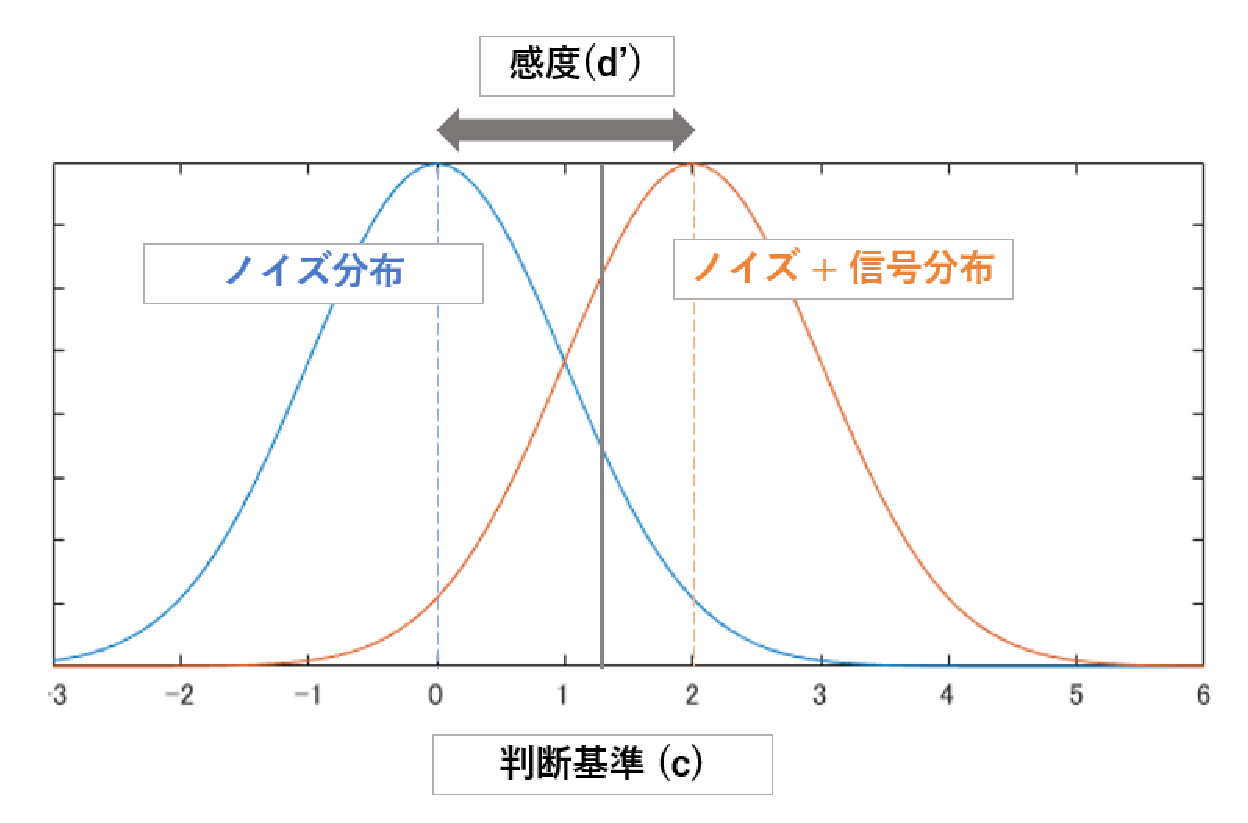
\includegraphics[width=15cm]{../figures/sdt.eps}
  \caption{信号検出理論で仮定する二つの正規分布}
\end{figure}

二つの分布が分かり,被験者ごとの判断基準(例...合計値が10以上だったらYes)が分かってしまえば,先程の表にあったヒッ
ト率やミス率も計算できます.単に分布を二つ並べて,線を引いて,線の右左のどちら側かと,本来はどっちの分布に含まれているかで4パターンに分けられますからね.これがそれぞれ先程の4指標に対応しているわけです.\\
 図にすると以下(図\ref{im:sdt2}, \ref{im:sdt3})のようになります.Hit, Miss, False Alarm, Correct Rejection のそれぞれがどちらの分布に属していて,どちらの分布として判定されたのかを確認してください.


\begin{figure}
  \label{im:sdt2}
  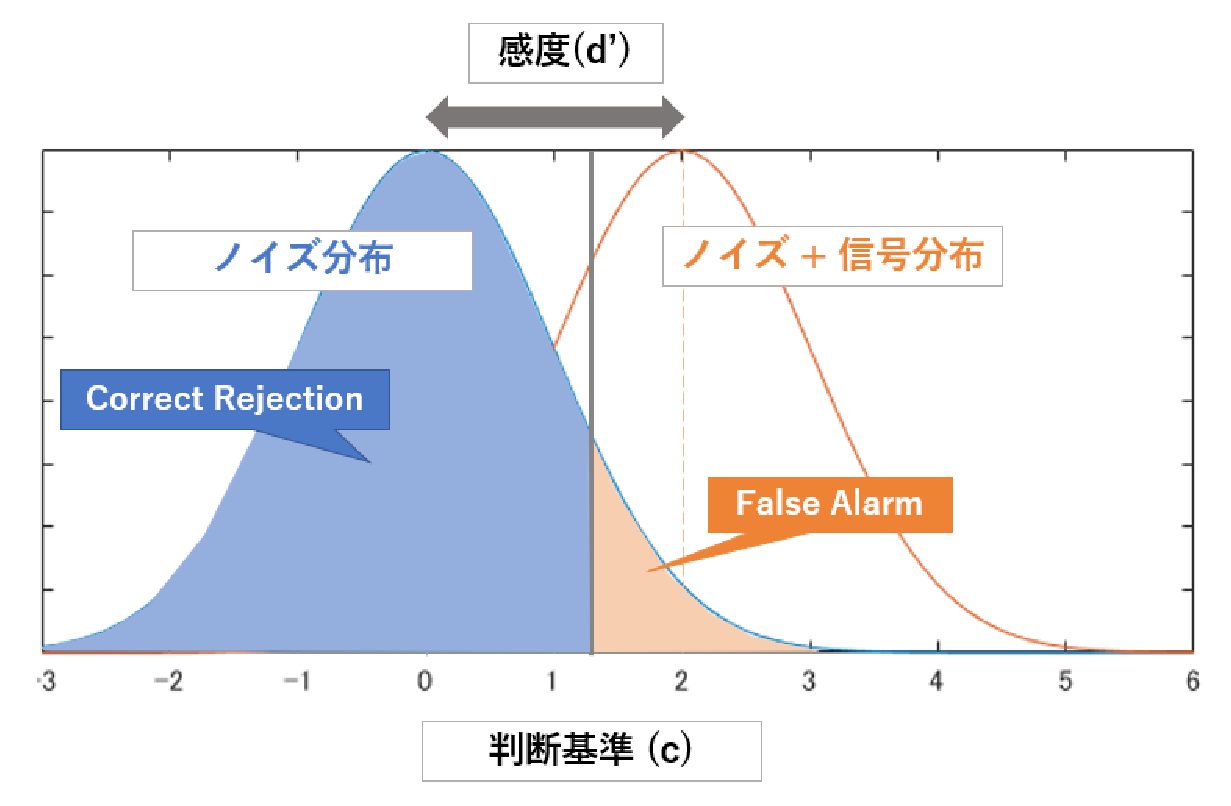
\includegraphics[width=15cm]{../figures/CR-FA.eps}
  \caption{ノイズ分布の二つの領域}
\end{figure}

\begin{figure}
  \label{im:sdt3}
  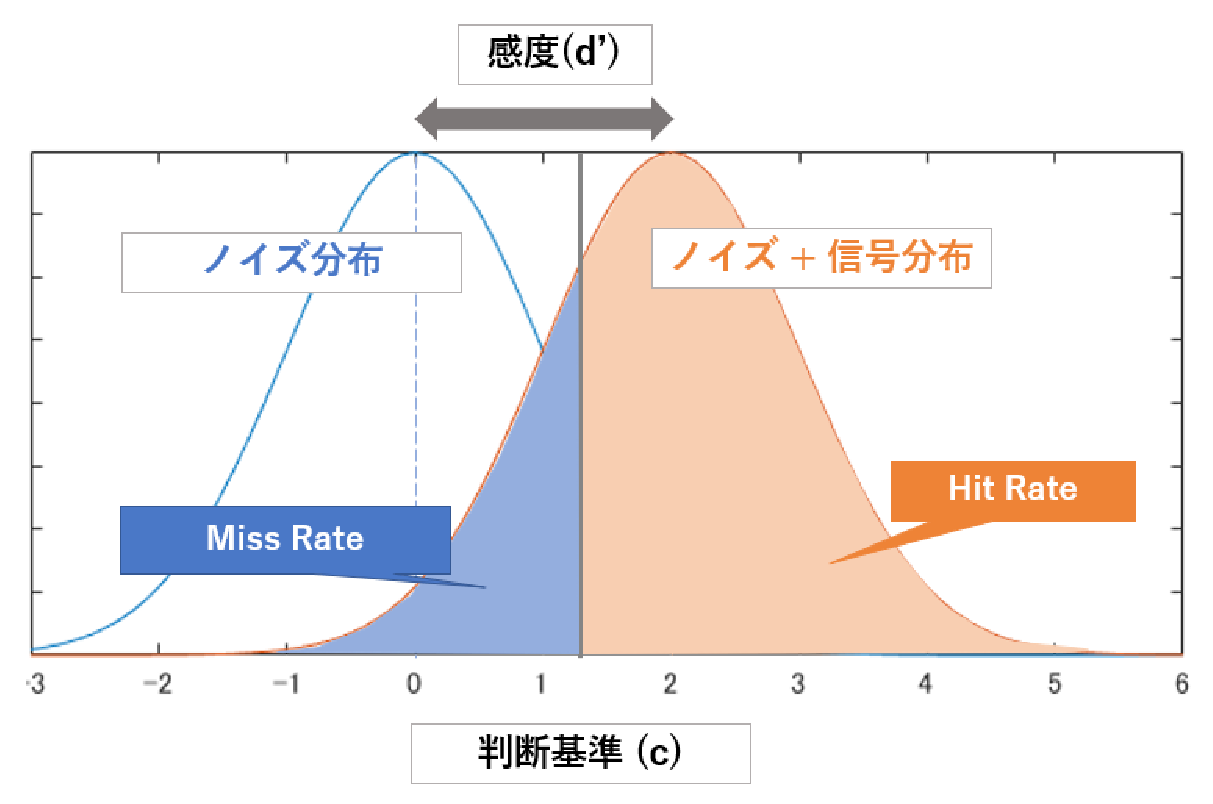
\includegraphics[width=15cm]{../figures/HR-MR.eps}
  \caption{信号分布の二つの領域}
\end{figure}


では逆に考えると,4指標の値が分かれば二つの分布(の距離)も判断基準も推定できる事になります.この,分布間の距離を感度(d'),判断基準を反応バイアス(c)として推定するのが信号検出理論です.

それぞれ算出法を考えます.感度は定義上は分布の距離なので

\begin{eqnarray}
  d' = \frac{\mu_{s+n}-\mu_n}{\sigma_n}
\end{eqnarray}

となります.これはノイズ+信号分布とノイズ分布の平均の差をノイズ分布の標準偏差で割るということで,つまり分布間の距離がノイズ分布の標準偏差何個分に相当するのかの指標です.多くの場合,ノイズ分布は標準偏差が1の正規分布を仮定するので,その場合は単純に平均の差を意味します.こうして算出される感度(d')は,二つの分布に対する被験者の心的距離です.区別しやすいもの程距離は離れていて,つまり感度も高くなります.いわゆる"優秀"な成績は感度が高い状態ですね.これは分布間の距離なので,被験者が積極的か保守的かなどの判断基準(c)の影響を受けない弁別能力を反映している事が分かるかと思います.\\

\subsection{感度}
感度は刺激が強く(極端に)なればなるほど高くなるし,学習によっても高くなる傾向があります.実際の場では,より正確には分布の平均位置を出すのは難しいので次のようなステップで感度を求めます.

まず,信号分布に対するヒット率(ヒットとミスの割合)と,ノイズ分布に対する誤警報率(CRとFAの割合)を算出します.これは以下の式で得られます.

\begin{eqnarray}
  \text{ヒット率} = p(yes|SN)= \frac{\text{ヒット数}}{\text{ヒット数} + \text{ミス数}}\\
  \text{誤警報率} = p(yes|N) = \frac{\text{誤警報数}}{\text{誤警報数} + \text{正棄却数}}
\end{eqnarray}

これらは,それぞれ判断基準より上の信号分布,ノイズ分布の面積に相当します.ノイズ分布と信号分布は平均が違うだけで同形の分布だったので,標準正規分布において右側の面積を積分すると計算したヒット率や誤警報率になる点をそれぞれ求めてやれば,その数値の差はすなわち分布の平均の差と等しくなる事が分かるかと思います.図(\ref{im:sdt2}, \ref{im:sdt3})のオレンジの部分を比較してみてください.同じ灰色の線(判断基準)に対し,オレンジ部分はかなり異なりますね.この差がすなわち分布間の距離ということです.よって以下の計算をします.

\begin{eqnarray}
  d' = Z(\text{ヒット率}) - Z(\text{誤警報率})
\end{eqnarray}

ここで,Z()はZ得点です.z得点とは,標準正規分布の平均を基準にした標準偏差数です.その分布の平均からどれだけ離れているかですね.これを二つの分布それぞれについて算出し,その差を求める事で分布間の距離を測るわけです.Zを取らないといけない理由は,そもそも独立な異なる分布を比較する際には標準化する必要があったのでしたね.

\begin{lstlisting}[caption=感度の計算,label=sc:sdt1]
  dat_ph = hit / (hit + miss);
  dat_pf = fa  / (fa  + cr);
  d' = norminv(dat_ph) -norminv(dat_pf);
\end{lstlisting}

こうして得られた感度は,大きい値であるほどしっかりとノイズ分布と信号分布を区別できるという事になります.これを使って,Aの被験者とBの被験者のどちらが性格にYesと答えられているかといったような事が分かりますね.

\subsection{反応バイアス}
反応バイアスは,被験者がそもそもYes/Noのどちらかに偏って答えやすいかどうかの指標です.「Yesをうまく検知できたら報酬をあげます」とか,「なるべく間違ってYesと答えないでください」といった指示が実験者から与えられていたり,本人の性格だったりによってどちらに答えやすいかは被験者ごとに異なります.感度はこのバイアスの影響を受けない指標だったわけですが,バイアス自体は以下のようにして求めれます.

\begin{eqnarray}
  C = \frac{1}{2} (Z(\text{ヒット率} + \text{誤警報率}))
\end{eqnarray}

これは,それぞれの分布の平均が判断基準からどれだけ離れているかの値(Z())の平均です.簡単ですね.この値が負だと被験者はYesと答えやすく,正だとNoと答えやすい,そして0だとバイアスがないという事になります.\\
\\
\subsection{まとめ}
信号検出理論は様々な知覚実験に利用できます.たとえば,ある特定の刺激パターン(音でも光でも顔画像でも)を学習し,それを検知したらYesと答えるといった課題はよく見られると思います.これを単純に正答率で評価してしまうと,被験者によって様々な反応バイアスがあるためにあまり正しくない評価になりかねません.そういう時に感度を計算すると便利ですね.そうする事で,たとえば疾患患者は感度が著しく低く,反応バイアスは健常者と変わらないとかそういった議論ができるようになるわけですね.


\begin{thebibliography}{99}
%はじめに
 \bibitem{radio} Lazepnik, Y. (2002). ``Can a biologist fix a radio?-Or, what I learned while studying apoptosis.'' Cancer Cell, 2(3), 179-182.
 \bibitem{Jonas} Jonas, Eric, and Konrad Paul Kording. (2017). "Could a neuroscientist understand a microprocessor?." PLoS computational biology 13.1.
 \bibitem{mar} Marr. (1982). ``Vision.'' 
 
 %情報理論
 \bibitem{fep} Friston, K. (2010). ``The free-energy principle: A unified brain theory?'' Nature Reviews Neuroscience. Volume 11, Issue 2, February 2010, 127-138
 \bibitem{tort} Adriano B. L. Tort, et al. (2010). ``Measuring Phase-Amplitude Coupling Between Neuronal Oscillations of Different Frequencies'' Journal of Neurophysiolosy 104:1195-1210.
 \bibitem{prml} Christopher M. Bishop. (2006). ``Pattern Recognition and Machine Learning''
 \bibitem{distance} Wikipedia
 \bibitem{dist} yumaloop. ``Kullback-Leibler Divergenceについてまとめる'' https://yul.hatenablog.com/entry/2019/01/07/152738
 \bibitem{kitano} Katunori Kitano. ``Transfer entropyを用いた神経回路の解析'' Annual Review 神経 2017 I.Basic Neuroscience.
\end{thebibliography}
\end{document}